%-----------------------------------------------------------------
%	BASIC DOCUMENT LAYOUT
%-----------------------------------------------------------------
\documentclass[paper=a4, fontsize=12pt, twoside=semi, abstracton, listof=totoc, toc=left]{scrartcl}
\usepackage[T1]{fontenc}
\usepackage[utf8]{inputenc}
\usepackage{lmodern}
\usepackage{slantsc}
\usepackage{microtype}
\usepackage[british]{babel}
% \usepackage[backend=bibtex, style=phys, sorting=none, citestyle=authoryear, maxbibnames=3, maxcitenames=2]{biblatex}
\usepackage[backend=bibtex, style=trad-abbrv, sorting=none, maxbibnames=3, maxcitenames=2]{biblatex}
\addbibresource{OpenData.bib}
\makeatletter
	\def\blx@maxline{77}
\makeatother

% Sectioning layout
\addtokomafont{sectioning}{\normalfont\scshape}
\usepackage{tocstyle}
\usetocstyle{standard}
\renewcommand*\descriptionlabel[1]{\hspace\labelsep\normalfont\bfseries{#1}}
\usepackage[titletoc]{appendix}

% Empty pages
\usepackage{etoolbox}
% \pretocmd{\toc}{\cleardoubleevenemptypage}{}{}
% \pretocmd{\section}{\cleardoubleevenemptypage}{}{}
\pretocmd{\part}{\cleardoubleevenemptypage\thispagestyle{empty}}{}{}
\renewcommand\partheadstartvskip{\clearpage\null\vfil}
\renewcommand\partheadmidvskip{\par\nobreak\vskip 20pt\thispagestyle{empty}}

% Paragraph indentation behaviour
\setlength{\parindent}{0pt}
\setlength{\parskip}{0.3\baselineskip plus2pt minus2pt}
\newcommand{\sk}{\medskip\noindent}

% Fancy header and footer
\usepackage{fancyhdr}
\pagestyle{fancyplain}
\fancyhead[LO]{\thepage}
\fancyhead[CO]{}
\fancyhead[RO]{\nouppercase{\mytitle}}
\fancyhead[LE]{\nouppercase{\rightmark}}
% \fancyhead[LE]{\nouppercase{\leftmark}}
\fancyhead[CE]{}
\fancyhead[RE]{\thepage}
\fancyfoot{}
\renewcommand{\headrulewidth}{0.3pt}
\renewcommand{\footrulewidth}{0pt}
\setlength{\headheight}{13.6pt}

%-----------------------------------------------------------------
%	MATHS AND SCIENCE
%-----------------------------------------------------------------
\usepackage{amsmath,amsfonts,amsthm,amssymb}
\usepackage{xfrac}
\usepackage[a]{esvect}
\usepackage{chemformula}
\usepackage{graphicx}

\usepackage[arrowdel]{physics}
	\renewcommand{\vnabla}{\vec{\nabla}}
	% \renewcommand{\vectorbold}[1]{\boldsymbol{#1}}
	% \renewcommand{\vectorarrow}[1]{\vec{\boldsymbol{#1}}}
	% \renewcommand{\vectorunit}[1]{\hat{\boldsymbol{#1}}}
	\renewcommand{\vectorarrow}[1]{\vec{#1}}
	\renewcommand{\vectorunit}[1]{\hat{#1}}
	\renewcommand*{\grad}[1]{\vnabla #1}
	\renewcommand*{\div}[1]{\vnabla \vdot \va{#1}}
	\renewcommand*{\curl}[1]{\vnabla \cp \va{#1}}
	\let\rot\curl

% SI units
\usepackage[separate-uncertainty=true]{siunitx}
% \sisetup{range-phrase = \text{--}, range-units = brackets}
\sisetup{range-phrase = \text{--}, range-units = single}
\DeclareSIPrePower\quartic{4}
	%\DeclareSIUnit\micron{\micro\metre}

% Smaller trig functions
\newcommand{\Sin}{\trigbraces{\operatorname{s}}}
\newcommand{\Cos}{\trigbraces{\operatorname{c}}}
\newcommand{\Tan}{\trigbraces{\operatorname{t}}}

% Operator-style notation for matrices
\newcommand*{\mat}[1]{\hat{#1}}

% Matrices in (A|B) form via [c|c] option
\makeatletter
\renewcommand*\env@matrix[1][*\c@MaxMatrixCols c]{%
  \hskip -\arraycolsep
  \let\@ifnextchar\new@ifnextchar
  \array{#1}}
\makeatother

% Shorter \mathcal and \mathbb
\newcommand*{\mc}[1]{\mathcal{#1}}
\newcommand*{\mbb}[1]{\mathbb{#1}}

% Shorter ^\ast and ^\dagger
\newcommand*{\sast}{^{\star}{}}
\newcommand*{\sdag}{^{\dagger}{}}

% Blackboard bold identity
\usepackage{bbm}
\newcommand*{\bbid}{\mathbbm{1}}

% Shorter displaystyle
\newcommand*{\dsp}{\displaystyle}

% Inexact differential
\newcommand{\dbar}{\mathchar'26\mkern-12mu\mathrm{d}}
\newcommand{\indd}[1]{\dbar{#1}}

% Arrows with text and cancels for developments
\newcommand{\tikzmark}[1]{\tikz[overlay,remember picture] \node (#1) {};}
\tikzset{square arrow/.style={to path={-- ++(0,-.25) -| (\tikztotarget)}}}
\usepackage{cancel}

\newcommand*\acr[1]{\textscale{.85}{#1}}

%-----------------------------------------------------------------
%	OTHER PACKAGES
%-----------------------------------------------------------------
\usepackage{environ}

%Left numbered equations
\makeatletter
	\NewEnviron{Lalign}{\tagsleft@true\begin{align}\BODY\end{align}}
\makeatother

% Plots and graphics
\usepackage{pgfplots}
\usepackage{tikz}
\usepackage{color}
	\makeatletter
		\color{black}
		\let\default@color\current@color
	\makeatother

% Richer enumerate, figure, and table support
\usepackage{enumerate}
\usepackage[shortlabels]{enumitem}
\usepackage{float}
\usepackage{tabularx}
\usepackage{booktabs}
	%\setlength{\intextsep}{8pt}
% \numberwithin{equation}{section}
% \numberwithin{figure}{section}
% \numberwithin{table}{section}

% No indentation after certain environments
\makeatletter
\newcommand*\NoIndentAfterEnv[1]{%
	\AfterEndEnvironment{#1}{\par\@afterindentfalse\@afterheading}}
\makeatother
%\NoIndentAfterEnv{thm}
\NoIndentAfterEnv{defi}
\NoIndentAfterEnv{example}
\NoIndentAfterEnv{table}

% Misc packages
\usepackage{ccicons}
\usepackage{lipsum}
\usepackage{todonotes}
\usepackage{array}
\usepackage{multirow}

% Print DOI only if there's no URL
\renewbibmacro*{doi+eprint+url}{%
  \iftoggle{bbx:doi}
    {\iffieldundef{url}{\printfield{doi}}{}}
    {}%
  \newunit\newblock
  \iftoggle{bbx:eprint}
    {\usebibmacro{eprint}}
    {}%
  \newunit\newblock
  \iftoggle{bbx:url}
    {\usebibmacro{url+urldate}}
    {}}

%-----------------------------------------------------------------
%	SYNTAX HIGHLIGHTING
%-----------------------------------------------------------------
\usepackage[formats]{listings}
\usepackage{relsize}
\usepackage{chngcntr}

\renewcommand{\lstlistingname}{Snippet}
\renewcommand{\lstlistlistingname}{List of snippets}

\lstloadlanguages{R}
\lstdefinelanguage{Renhanced}[]{R}{%
	morekeywords={acf,ar,arima,arima.sim,colMeans,colSums,is.na,is.null,%
	mapply,ms,na.rm,nlmin,replicate,row.names,rowMeans,rowSums,seasonal,%
	sys.time,system.time,ts.plot,which.max,which.min,%
	rename,mutate,unite,select,filter,left_join,group_by,dplyr::select,%
	ggplot,aes,geom_line,geom_hline,geom_point,geom_path,geom_errorbar,%
	geom_abline,geom_smooth%
	geom_cartogram,coord_proj,scale_x_longitude, scale_y_latitude,%
	labs,guides,annotate,theme,rowwise,%
	scale_linetype_manual,scale_colour_manual,scale_x_log10,scale_y_log10,%
	attr,paste,paste0,bind_rows,str_trim,as.numeric,as.dataframe,data.frame},
	deletekeywords={c,range,step},
	alsoletter={.,_,::},
	otherkeywords = {!,!=,~,\$,*,\&,\%/\%,\%*\%,\%\%,\%>\%,<-,<<-,\% in \%}
	}

\newcommand*{\inline}{\lstinline[basicstyle=\normalsize\ttfamily]}


\lstset{language=C,
		frame=tb,
		% captionpos=b,
		tabsize=2,
		% showtabs=true,
		breaklines=true,
		breakatwhitespace=true,
		basicstyle=\smaller\ttfamily,
		numbers=left,
		numberstyle=\tiny,
		numbersep=7.5pt,
		% commentstyle=\textsl,
		xleftmargin=3ex}
\lstset{escapeinside={(*}{*)}}   % for (*\ref{ }*) inside lstlistings (Scode)

\usepackage{xcolor}
\newcommand\crule[3][black]{\textcolor{#1}{\rule{#2}{#3}}}
\definecolor{mypurple}{RGB}{147, 34, 156}
\definecolor{mypink}{RGB}{255, 0, 110}
\definecolor{myblue}{RGB}{69, 57, 252}
\definecolor{myorange}{RGB}{246, 149, 50}
\definecolor{mygreen}{RGB}{73, 166, 87}

%-----------------------------------------------------------------
%	THEOREMS
%-----------------------------------------------------------------
\usepackage{thmtools}

% Theroems layout
\declaretheoremstyle[
	spaceabove=6pt, spacebelow=6pt,
	headfont=\normalfont,
	notefont=\mdseries, notebraces={(}{)},
	bodyfont=\small,
	postheadspace=1em,
]{small}

\declaretheorem[style=plain,name=Theorem,qed=$\square$,numberwithin=section]{thm}
\declaretheorem[style=plain,name=Corollary,qed=$\square$,sibling=thm]{cor}
\declaretheorem[style=plain,name=Lemma,qed=$\square$,sibling=thm]{lem}
\declaretheorem[style=definition,name=Definition,qed=$\blacksquare$,numberwithin=section]{defi}
\declaretheorem[style=definition,name=Example,qed=$\blacktriangle$,numberwithin=section]{example}
\declaretheorem[style=small,name=Proof,numbered=no,qed=$\square$]{sproof}

%-----------------------------------------------------------------
%	ELA MOTHERFUCKING GEMINADA
%-----------------------------------------------------------------
\def\xgem{%
	\ifmmode
		\csname normal@char\string"\endcsname l%
	\else
		\leftllkern=0pt\rightllkern=0pt\raiselldim=0pt
		\setbox0\hbox{l}\setbox1\hbox{l\/}\setbox2\hbox{.}%
		\advance\raiselldim by \the\fontdimen5\the\font
		\advance\raiselldim by -\ht2
		\leftllkern=-.25\wd0%
		\advance\leftllkern by \wd1
		\advance\leftllkern by -\wd0
		\rightllkern=-.25\wd0%
		\advance\rightllkern by -\wd1
		\advance\rightllkern by \wd0
		\allowhyphens\discretionary{-}{}%
		{\kern\leftllkern\raise\raiselldim\hbox{.}%
			\kern\rightllkern}\allowhyphens
	\fi
}
\def\Xgem{%
	\ifmmode
		\csname normal@char\string"\endcsname L%
	\else
		\leftllkern=0pt\rightllkern=0pt\raiselldim=0pt
		\setbox0\hbox{L}\setbox1\hbox{L\/}\setbox2\hbox{.}%
		\advance\raiselldim by .5\ht0
		\advance\raiselldim by -.5\ht2
		\leftllkern=-.125\wd0%
		\advance\leftllkern by \wd1
		\advance\leftllkern by -\wd0
		\rightllkern=-\wd0%
		\divide\rightllkern by 6
		\advance\rightllkern by -\wd1
		\advance\rightllkern by \wd0
		\allowhyphens\discretionary{-}{}%
		{\kern\leftllkern\raise\raiselldim\hbox{.}%
			\kern\rightllkern}\allowhyphens
	\fi
}

\expandafter\let\expandafter\saveperiodcentered
	\csname T1\string\textperiodcentered \endcsname

\DeclareTextCommand{\textperiodcentered}{T1}[1]{%
	\ifnum\spacefactor=998
		\Xgem
	\else
		\xgem
	\fi#1}

%-----------------------------------------------------------------
%	DEDICATION ENVIRONMENT
%-----------------------------------------------------------------

\newenvironment{mydedication}
	{\clearpage           % we want a new page
	\thispagestyle{empty}% no header and footer
	\vspace*{\stretch{1}}% some space at the top
	\itshape             % the text is in italics
	\raggedleft          % flush to the right margin
	}
	{\par % end the paragraph
	\vspace{\stretch{3}} % space at bottom is three times that at the top
	\clearpage           % finish off the page
	}

%-----------------------------------------------------------------
%	PDF INFO AND HYPERREF
%-----------------------------------------------------------------
\usepackage{hyperref}
\hypersetup{colorlinks, citecolor=black, filecolor=black, linkcolor=black, urlcolor=black}
\usepackage{cleveref}
	\crefname{section}{\S}{\SS}
	\Crefname{section}{\S}{\SS}
	\crefname{listing}{snippet}{}

\newcommand*{\mytitle}{Parallel Programming: OpenMP}
\newcommand*{\mysubtitle}{Assignment 2}
\newcommand*{\myauthor}{Alfredo Hernández \and Alejandro Jiménez}
% \newcommand*{\mysupervisor}{J. Minguillón}
% \newcommand*{\mytutor}{}
\newcommand*{\myuni}{Universitat Autònoma de Barcelona}
\newcommand*{\mydate}{28th November}

\pdfstringdefDisableCommands{\def\and{and }}

\usepackage{hyperxmp}
\hypersetup{pdfauthor={\myauthor}, pdftitle={\mytitle: \mysubtitle}}

%-----------------------------------------------------------------
%	TITLE SECTION AND DOCUMENT BEGINNING
%-----------------------------------------------------------------
\newcommand{\horrule}[1]{\rule{\linewidth}{#1}}
\title{
	\normalfont
	\small \scshape{\myuni} \\ [25pt]
	\horrule{0.5pt} \\ [0.4cm]
	\huge \mytitle \\
	\Large \scshape{\mysubtitle} \\
	\horrule{2pt} \\ [0.5cm]
}
\author{\myauthor }
% \\ \footnotesize Supervised by: \mysupervisor \\ \footnotesize Academic tutor: \mytutor}
\date{\mydate}

\begin{document}

%\counterwithin{lstlisting}{section}

\clearpage\maketitle
\thispagestyle{empty}
\addtocounter{page}{-1}

%-----------------------------------------------------------------
%	DEDICATION
%-----------------------------------------------------------------
% \begin{mydedication}
% 	Dedicated to RMT, Val \& the Brotherhood
% \end{mydedication}

%-----------------------------------------------------------------
%	DOCUMENT BODY
%-----------------------------------------------------------------
% \cleardoubleevenemptypage
\include{./contents/0-abstract}

\pdfbookmark[1]{\contentsname}{toc}
\tableofcontents

%-----------------------------------------------------------------
%	INTRODUCTION
%	!TEX root = ./../main.tex
%-----------------------------------------------------------------
\section{Introduction}

In this assignment we aim to improve the execution time of the now-common Laplace 2D code and measure the impact of using MPI.

In order to make the biggest difference on the code and fully appreciate the power of parallel computing, we chose the most computational demanding loop and created many threads using OpenMP, which would split the iterations into different, parallel, more efficient processes. Nextly, we would add MPI orders in as many loops as we did found useful. 

Eventually, We will measure the impact of the parallelisation of the code using and more sophisticated analytical tools such as \emph{TAU}. Using \emph{TAU} we will try to identify and analyse the different internal operations of the code and how their performance varies when using a different number of threads.


% Moreover, we tested different numbers of threads and many scheduling methods.

% Finally, we recorded the execution times for every alteration in the paralleling in order to be able to compare different paralleling metodologies and decide which method performed the better on our code.



%-----------------------------------------------------------------
%	PERFORMANCE
%	!TEX root = ./../main.tex
%-----------------------------------------------------------------
\section{Analysis}

\subsection{Setting up the system before working}

Before doing anything, we need to load the \inline{modules} of the compiler and libraries we have to use:
\begin{lstlisting}
module load gcc/6.1.0
module load papi/5.4.3
module load openmpi/1.8.1
\end{lstlisting}

After installing TAU and compiling the different \inline{Makefile}s, we need to make sure we include the installation directory on the \inline{$PATH}, this can be done on each session (or by modifying the \inline{.bash_profile}:
\begin{lstlisting}
export PATH=/home/master/ppM/ppM-1-10/my_TAU/x86_64/bin:$PATH
\end{lstlisting}

%-----------------------------------------------------------------
\subsection{Parallelisation with OpenMP}

One of the main variables to consider when improving the performance of a code using OpenMP is the number of threads that we use. Specifying the exact number of threads to be used can be done easily using this command on our source C code:

\begin{lstlisting}
#pragma omp parallel for num_threads(NUM_THREADS)
\end{lstlisting}

This can improve greatly the performance of the code when used on sequential portions of the program, such as loops where each step is independent from the others.

In \cref{sn:omp} we can see how we've implemented the \inline{#pragma} to select the amount of threads we want to use in our program:

\begin{lstlisting}[firstnumber=17, label=sn:omp, caption= Example of parallelisation on nested loops using OpenMP]
float laplace_step(float *in, float *out, int n)
{
  int i, j;
  float error=0.0f;
  #pragma omp parallel for num_threads(NUM_THREADS)
  for ( j=1; j < n-1; j++ )
    #pragma omp simd reduction(max:error)
    for ( i=1; i < n-1; i++ )
    {
      out[j*n+i]= stencil(in[j*n+i+1], in[j*n+i-1], in[(j-1)*n+i], in[(j+1)*n+i]);
      error = max_error( error, out[j*n+i], in[j*n+i] );
    }
  return error;
}
\end{lstlisting}

Where \inline{NUM_THREADS} is an integer that depends on the architecture of the machine that we are using. In our case, we used 2, 4, and 8 threads.

To compile the code we just use vanilla \inline{gcc} with the appropriate flags to enable OpenMP:
\begin{lstlisting}
gcc -lm -fopenmp -o test_Np lapFusion.c
\end{lstlisting}
where \inline{N} is 2, 4, or 8.

For this first measure of performance, we have used the widely known tool \inline{perf stat} on a code that computes the Laplace 2D equation on a $512 \times 512$ matrix with $500$ iterations:

\begin{lstlisting}
perf stat ./test_Np 512 500
\end{lstlisting}

\bigskip
The results shown in table \ref{tab:perf-stat} reflect an improvement of the performance when using an increasing amount of threads, as expected.

\begin{table}[H]
\centering
\begin{tabular}{c c}
    \toprule
    \toprule
    \textbf{Num. Threads} & \textbf{Run Time} \\
    \midrule
    No parallel           & \SI{4.841}{\s}    \\
    2 Threads             & \SI{2.521}{\s}    \\
    4 Threads             & \SI{1.685}{\s}    \\
    8 Threads             & \SI{0.948}{\s}    \\
    \bottomrule
\end{tabular}
\caption{Run time obtained on multiple threads}
\label{tab:perf-stat}
\end{table}

It is crucial to notice that the more threads we use the more efficient the computation becomes, and by a large difference; this fact reflects the great importance of parallelisation and its implications on high-performance computation.

%-----------------------------------------------------------------
\subsection{Analysis with TAU}

Up to this point we have seen a superficial picture of how the performance increases using OpenMP as a tool to parallelise the code. Now we are going to use \emph{TAU}, a toolkit for analysis performance that allows us to study in detail the performance of many parts of the code that we have parallelised.

As a comparison, we have used the same code as before with the same number of iterations and problem size.

%-----------------------------------------------------------------
\subsubsection{Using profile files (\texttt{paraprof})}

The toolkit \inline{paraprof} (bundled with TAU) allows us to parallel profile analysis. This is similar to using \inline{perf stat}, but now we have data for each of the threads.

For this part, we need to set the following environment variables:
\begin{lstlisting}
export TAU_MAKEFILE=$HOME/my_TAU/x86_64/lib/Makefile.tau-openmp-opari
export TAU_OPTIONS=-optCompInst
export TAU_PROFILE=1
\end{lstlisting}

Then we have to compile our source code using TAU, and then run it as usual
\begin{lstlisting}
tau_cc.sh -lm -o openmp.test_Np_trace lapFusionN.c
./openmp.test_Np_trace 512 500
\end{lstlisting}
where \inline{N} can be 2, 4, or 8.

This will give us \inline{profile.0.0.*} profile files; one for each of the threads used. To read and analyse these files we can use the \inline{paraprof} tool.

\bigskip
Even though we have run the same code, the first thing we notice here is an increase on the \emph{Run Time}. This happens because now we are asking for an on-time measurement of the performance of the code on internal steps; this is more computationally demanding than a simple \inline{perf stat} and thus it takes more time to compute it.

In figure \ref{fig:paraprof-example} we can see the typical 3D Visualisation of the \inline{TIME} metric using \inline{paraprof}. The height of the bars represents the metric, whilst on the $Y$ axis we have the different functions of the compiled code. We will focus on the time metric of the \inline{parallelfor} functions.

\begin{figure}[H]
	\centering
	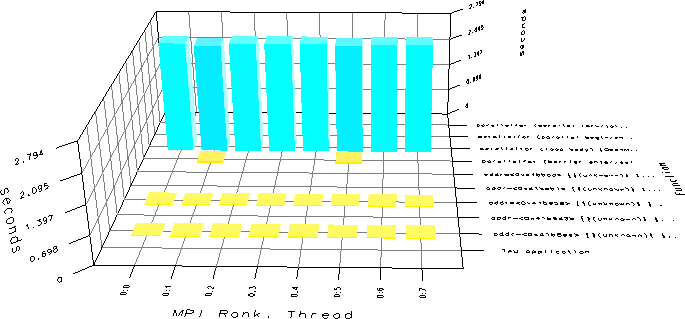
\includegraphics[width=0.95\textwidth]{images/paraprof-example}
	\caption{3D Visualisation of the run time on 8 threads}
	\label{fig:paraprof-example}
\end{figure}

\begin{table}[H]
\centering
\begin{tabular}{l c c c}
    \toprule
    \toprule
    \textbf{Function} & \textbf{2 Threads} & \textbf{4 Threads} & \textbf{8 Threads} \\
    \midrule
    \texttt{parallelfor (barrier enter/exit)} & \SI{0.002}{\s} & \SI{0.007}{\s} & \SI{0.016}{\s} \\
    \texttt{parallelfor (loop body)}          & \SI{6.684}{\s} & \SI{5.65}{\s} & \SI{2.788}{\s} \\
    \texttt{parallelfor (parallel begin/end)} & \SI{0.00022}{\s} & \SI{0.00033}{\s} & \SI{0.00042}{\s} \\
    \texttt{parallelfor (parallel fork/join)} & \SI{0.001}{\s} & \SI{0.033}{\s} & \SI{0.002}{\s} \\
    \bottomrule
\end{tabular}
\caption{Run time obtained on multiple threads}
\label{my-label}
\end{table}

This table shows interesting results. On one hand we can see how the \emph{Run Time} of execution of some internal operations increases; such as \inline{barrier enter/exit}, \inline{parallel begin/end}, and \inline{parallel fork/join}. On the other hand we have an outstanding improvement of the performance of the main loop, the \inline{loop body} part; and this is important, for this is the more demanding part of the code and its performance improvement largely compensates the loss of speed on the others.


%-----------------------------------------------------------------
\subsubsection{Using traces (\texttt{jumpshot})}

Now that we have seen some of the standard measurement tools for parallelised code, we can explore even more detailed analytical tools.

For this part, we need to set the following environment variables:
\begin{lstlisting}
export TAU_MAKEFILE=$HOME/my_TAU/x86_64/lib/Makefile.tau-openmp-opari
export TAU_OPTIONS=-optCompInst
export TAU_TRACE=1
\end{lstlisting}

Then we have to compile our source code using TAU, and then run it as usual
\begin{lstlisting}
tau_cc.sh -lm -o openmp.test_Np_trace lapFusionN.c
./openmp.test_Np_trace 512 500
\end{lstlisting}
where \inline{N} can be 2, 4, or 8.

After doing this, we have to merge the obtained \inline{tautrace.0.0.*.trc} trace files into a readable \inline{.slog2} log file using the following commands:
\begin{lstlisting}
tau_treemerge.pl
tau2slog2 tau.trc tau.edf -o tauNthreads.slog2
\end{lstlisting}

To visualise the data of the logfile, we simply use the \inline{jumpshot} tool (also bundled with TAU):
\begin{lstlisting}
jumpshot tauNthreads.slog2
\end{lstlisting}

\bigskip
In tables \ref{tab:jump2}, \ref{tab:jump4}, and \ref{tab:jump8} we can see the results of the \inline{Category count}, \inline{Inclusive ratio}, and \inline{Exclusive ratio} obtained from the \inline{.slog2} log files for 2, 4, and 8 threads respectively.

We have selected to show only \inline{FLUSH} and the parallel operations of the program, to ease the analysis of the data. The \inline{FLUSH} operation deals with the different buffers of the program (temporary memory areas in which data is stored while it is being processed or transferred).

\begin{table}[H]
\centering
\begin{tabular}{c l c c c}
    \toprule
    \toprule
    \textbf{Legend} & \textbf{Function} & \textbf{\inline{count}} & \textbf{\inline{incl}} & \textbf{\inline{excl}} \\
    \midrule
    \crule[mypurple]{0.8cm}{0.3cm} & \texttt{FLUSH}                            & \num{12}   & \num{0.014} & \num{0.014} \\
    \crule[mypink]{0.8cm}{0.3cm}   & \texttt{parallelfor (barrier enter/exit)} & \num{1000} & \num{0.002} & \num{0.002} \\
    \crule[myblue]{0.8cm}{0.3cm}   & \texttt{parallelfor (loop body)}          & \num{1000} & \num{1.999} & \num{1.898} \\
    \crule[myorange]{0.8cm}{0.3cm} & \texttt{parallelfor (parallel begin/end)} & \num{1000} & \num{1.999} & \num{0}     \\
    \crule[mygreen]{0.8cm}{0.3cm}  & \texttt{parallelfor (parallel fork/join)} & \num{500}  & \num{1}     & \num{0}     \\
    \bottomrule
\end{tabular}
\caption{Data obtained from the logfile, using TAU with 2  threads}
\label{tab:jump2}
\end{table}

\begin{table}[H]
\centering
\begin{tabular}{c l c c c}
    \toprule
    \toprule
    \textbf{Legend} & \textbf{Function} & \textbf{\inline{count}} & \textbf{\inline{incl}} & \textbf{\inline{excl}} \\
    \midrule
    \crule[mypurple]{0.8cm}{0.3cm} & \texttt{FLUSH}                            & \num{24}   & \num{0.048} & \num{0.048} \\
    \crule[mypink]{0.8cm}{0.3cm}   & \texttt{parallelfor (barrier enter/exit)} & \num{2000} & \num{0.345} & \num{0.345} \\
    \crule[myblue]{0.8cm}{0.3cm}   & \texttt{parallelfor (loop body)}          & \num{2000} & \num{3.573} & \num{2.887} \\
    \crule[myorange]{0.8cm}{0.3cm} & \texttt{parallelfor (parallel begin/end)} & \num{2000} & \num{3.576} & \num{0.003} \\
    \crule[mygreen]{0.8cm}{0.3cm}  & \texttt{parallelfor (parallel fork/join)} & \num{500}  & \num{1}     & \num{0.058} \\
    \bottomrule
\end{tabular}
\caption{Data obtained from the logfile, using TAU with 4 threads}
\label{tab:jump4}
\end{table}

\begin{table}[H]
\centering
\begin{tabular}{c l c c c}
    \toprule
    \toprule
    \textbf{Legend} & \textbf{Function} & \textbf{\inline{count}} & \textbf{\inline{incl}} & \textbf{\inline{excl}} \\
    \midrule
    \crule[mypurple]{0.8cm}{0.3cm} & \texttt{FLUSH}                            & \num{48}   & \num{0.97}  & \num{0.97}  \\
    \crule[mypink]{0.8cm}{0.3cm}   & \texttt{parallelfor (barrier enter/exit)} & \num{4000} & \num{2.632} & \num{2.632} \\
    \crule[myblue]{0.8cm}{0.3cm}   & \texttt{parallelfor (loop body)}          & \num{4000} & \num{6.328} & \num{2.012} \\
    \crule[myorange]{0.8cm}{0.3cm} & \texttt{parallelfor (parallel begin/end)} & \num{4000} & \num{6.339} & \num{0.011} \\
    \crule[mygreen]{0.8cm}{0.3cm}  & \texttt{parallelfor (parallel fork/join)} & \num{500}  & \num{1}     & \num{0.222} \\
    \bottomrule
\end{tabular}
\caption{Data obtained from the logfile, using TAU with 8 threads}
\label{tab:jump8}
\end{table}

In figure \ref{fig:jumpshot-example} we can see an example of the Time Line of internal operations of each one of the used threads. Essentially, it reinforces the conclusions extracted from the previous section where we used \inline{paraprof} but it enables us to visualise the stats in more detail how each of the threads behaves by itself and in relation to the others.

\begin{figure}[H]
	\centering
	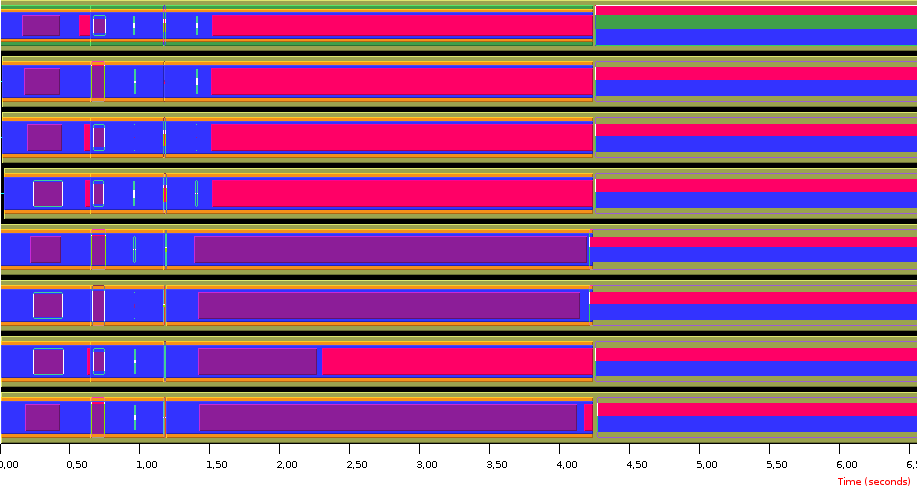
\includegraphics[width=\textwidth]{images/jumpshot-example}
	\caption{Time Line of the 8 threads visualised using an Identity Map}
	\label{fig:jumpshot-example}
\end{figure}

It is interesting to notice how Thread 0 is the one responsible to join the different threads after the parallel part of the program (initialisation of the matrix; see \cref{sn:omp}) is finished.

%-----------------------------------------------------------------
% \subsubsection{Using \texttt{PAPI}}

%-----------------------------------------------------------------
%	CONCLUSIONS
%	!TEX root = ./../main.tex
%-----------------------------------------------------------------
\section{Conclusions}

During the resolution of this exercise, we have had the opportunity to further improve the code of the first exercise of the course. This time, though, we have used a different methodology to paralellise the code, the widely employed \emph{OpenMP}. Moreover, we have got started in the analytical tool kits known as \emph{TAU} and we have learnt the basics to understand and interpret different visalisation techniques for performance measurement, profiling, and tracing on parallelised code.

All of this has let us understand the importance of parallel programming when aiming for high performance computation, for we have experienced the increase of performance in our code when applying such techniques.


% \begin{appendices}
% \include{./contents/A-code}
% \end{appendices}

%-----------------------------------------------------------------
%	BIBLIOGRAPHY
%-----------------------------------------------------------------


% \printbibliography[heading=bibintoc]
% \setcounter{secnumdepth}{0}
% \section{References}
% \printbibliography[title={Articles}, type=article, heading=subbibliography]
% \printbibliography[title={Books}, type=book, heading=subbibliography]
% \printbibliography[title={Websites}, type=online , heading=subbibliography]
% \printbibliography[title={Basic}, keyword=basic , heading=subbibliography]
% \printbibliography[title={Data Sets}, keyword=dataset , heading=subbibliography]
% \printbibliography[title={Licenses}, keyword=license , heading=subbibliography]

\end{document}
